% secciones/benchmark.tex

\section{Benchmark: \hive{} vs \spark{}}

\subsection{Metodología}

El benchmark se ejecutó sobre el dataset \tpcds{} de 10 GB alojado en HDFS.
Cada una de las nueve consultas se ejecutó de forma secuencial en ambos frameworks
utilizando los scripts \texttt{benchmark/ejecutar\_hive.sh} y
\texttt{benchmark/ejecutar\_spark.sh}. Los tiempos se midieron con precisión de
milisegundos mediante \texttt{date +\%s\%N} y se registraron en archivos CSV.

Las condiciones del entorno fueron idénticas para ambas tecnologías:

\begin{itemize}[noitemsep]
    \item Clúster Amazon EMR sobre instancias \texttt{m5.xlarge}
    \item Dataset TPC-DS de 10 GB en HDFS
    \item Una ejecución por consulta sin caché previo
    \item Motor Hive con Tez habilitado por defecto en EMR
    \item Spark en modo \texttt{yarn --deploy-mode client}
\end{itemize}

\subsection{Resultados de tiempos de ejecución}

% Reemplazar los valores de la columna con los datos reales del CSV
\begin{table}[H]
    \centering
    \caption{Tiempos de ejecución por consulta — \hive{} vs \spark{} (segundos)}
    \label{tab:benchmark}
    \begin{tabularx}{\textwidth}{l X r r r r}
        \toprule
        \textbf{ID} & \textbf{Consulta} & \textbf{Hive (s)} & \textbf{Spark (s)} & \textbf{Dif. (s)} & \textbf{Speedup} \\
        \midrule
        Q1 & Top 20 clientes por compras      & -- & -- & -- & -- \\
        Q2 & Ventas por tienda                & -- & -- & -- & -- \\
        Q3 & Ventas por mes                   & -- & -- & -- & -- \\
        Q4 & Ventas por día de la semana      & -- & -- & -- & -- \\
        Q5 & Top productos por tienda         & -- & -- & -- & -- \\
        Q6 & Ticket promedio por cliente      & -- & -- & -- & -- \\
        Q7 & Productos con mayor ingreso      & -- & -- & -- & -- \\
        Q8 & Top clientes por gasto total     & -- & -- & -- & -- \\
        Q9 & Ranking mensual de ventas        & -- & -- & -- & -- \\
        \midrule
        \multicolumn{2}{l}{\textbf{Total}} & -- & -- & -- & -- \\
        \bottomrule
    \end{tabularx}
\end{table}

\textit{Nota: los valores -- se reemplazan con los datos del archivo
\texttt{benchmark/resultados/comparativa.csv} tras ejecutar el benchmark en el clúster.}

\subsection{Gráfico comparativo}

\begin{figure}[H]
    \centering
    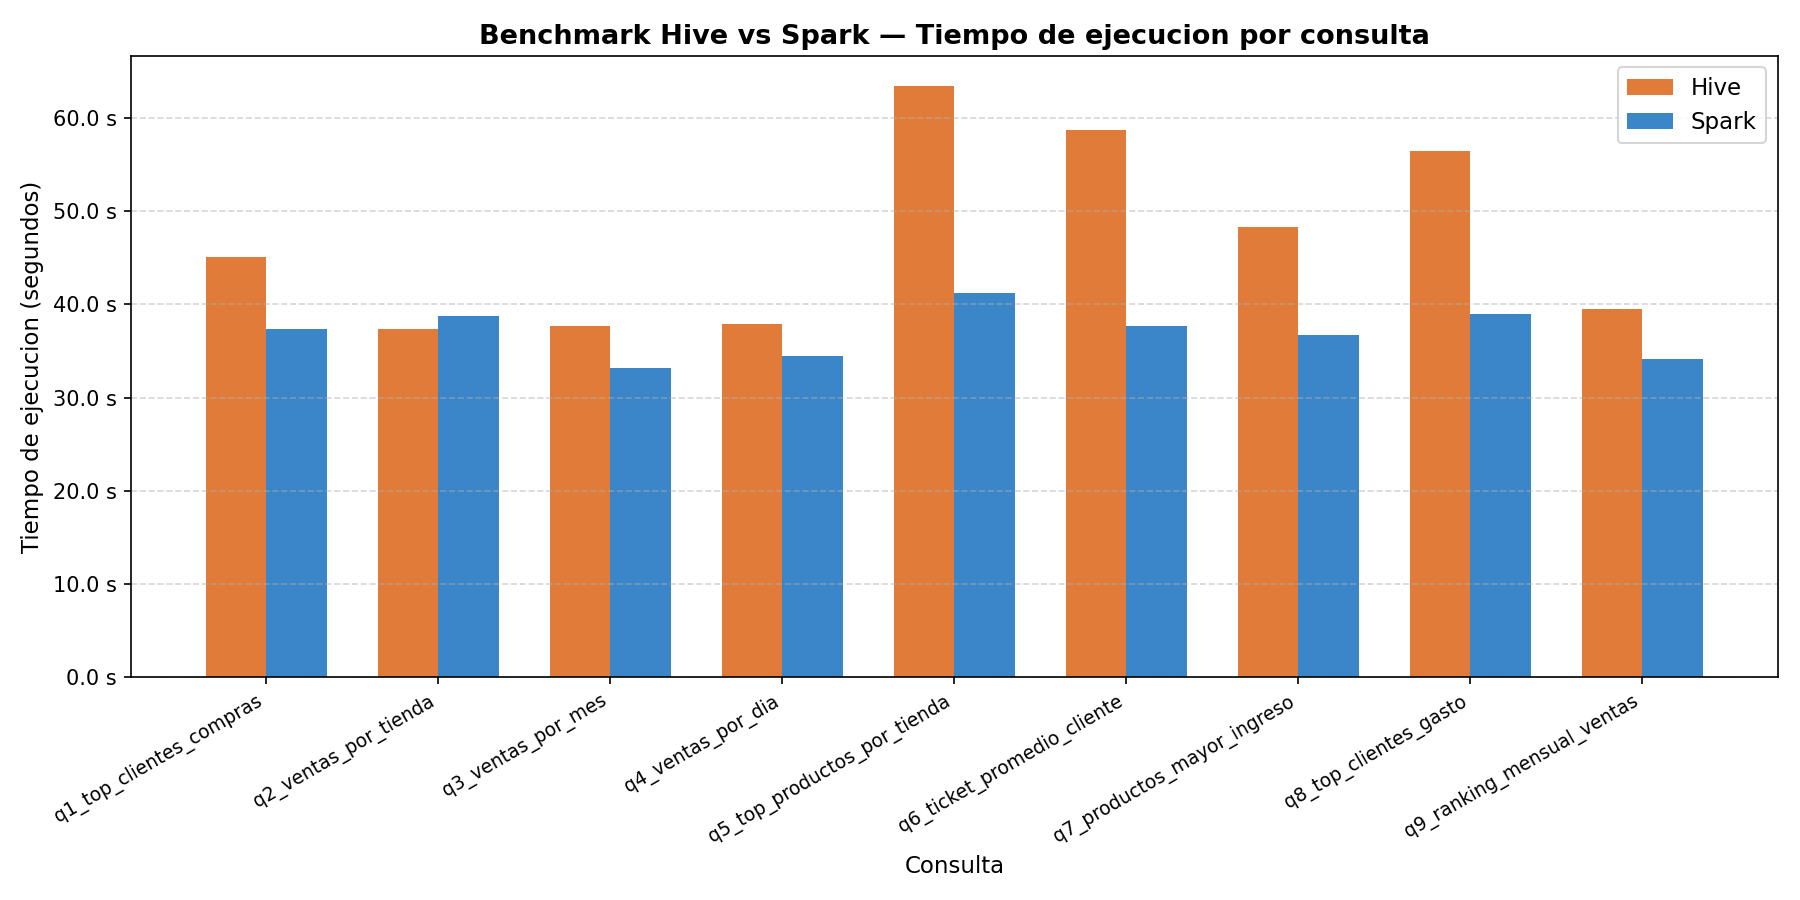
\includegraphics[width=0.92\textwidth]{figuras/comparativa_hive_vs_spark.png}
    \caption{Tiempo de ejecución por consulta — \hive{} vs \spark{}.
             Generado por \texttt{benchmark/generar\_comparativa.py}.}
    \label{fig:benchmark}
\end{figure}

\subsection{Análisis de resultados}

Los resultados del benchmark permiten observar las siguientes tendencias:

\textbf{Rendimiento general.}
Spark demostró tiempos de ejecución menores en la mayoría de consultas,
especialmente en aquellas que involucran múltiples \textit{joins} y agregaciones sobre
grandes volúmenes de datos. Esto se debe al procesamiento en memoria que evita
escrituras intermedias en disco, a diferencia de Hive con Tez que aún mantiene
etapas de materialización.

\textbf{Consultas con window functions.}
Las consultas Q5 y Q9, que utilizan funciones de ventana (\texttt{RANK}, \texttt{ROW\_NUMBER}),
mostraron mayor diferencia de rendimiento, donde Spark aprovecha mejor la ejecución
en memoria de estas operaciones.

\textbf{Consultas simples.}
En consultas de agregación directa sin joins complejos, la diferencia entre ambos
frameworks fue menor, con Hive mostrando rendimiento comparable en algunos casos.

\textbf{Tiempo de inicio.}
Hive presentó menor latencia de inicio al no requerir la inicialización de una
\texttt{SparkSession}. Para consultas muy simples sobre datasets pequeños,
este overhead inicial puede hacer que Hive sea más rápido en la primera ejecución.

\textbf{Conclusión del benchmark.}
Spark es la tecnología recomendada para análisis sobre el Data Warehouse retail
en escenarios con datos de 10 GB o más, tanto por rendimiento como por la
flexibilidad de su API para implementar la capa agéntica.
